\paragraph{Correlation coefficient}
To get correlation coefficient: convert each variable to standard units
and compute the average of their product.
\begin{center}
	$X,Y\text{: 2 RV}\Rightarrow \rho=\dfrac{Cov(X,Y)}{\sigma_{X}\sigma_{Y}}$
\end{center}
\begin{figure}[H]
	\begin{center}
		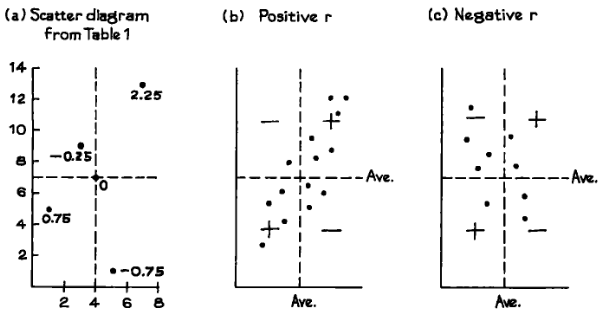
\includegraphics[width=.5\textwidth]{./chaps/17sec/images/correlationDiagram.png}
	\end{center}
	\caption{+: area where r is positive.\\-: area where r is 
	negative}
	\label{fig:7_correlationDiagram}
\end{figure}
Associated with each of one SD in $x$ there is an increase of only
$r$ SDs in $y$, on the average.
\begin{figure}[H]
	\begin{center}
		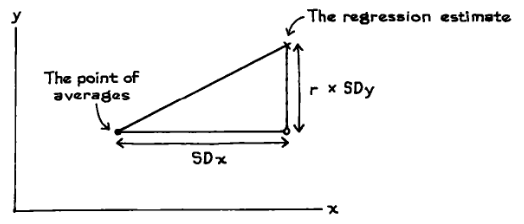
\includegraphics[width=.5\textwidth]{./chaps/17sec/images/2_correlDiag.png}
	\end{center}
	\caption{Graphical representation of $r$}
	\label{fig:2_correDiag}
\end{figure}
\begin{figure}[H]
	\begin{center}
		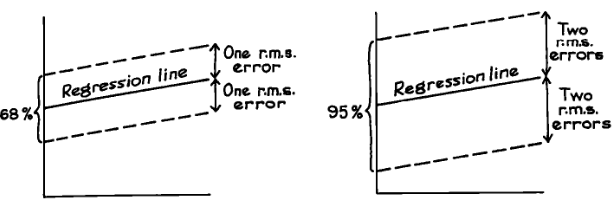
\includegraphics[width=.5\textwidth]{./chaps/17sec/images/3_residuals.png}
	\end{center}
	\caption{Graphical interpretation of Residual Mean Squares}
	\label{fig:3_rmsDiag}
\end{figure}
\paragraph{Property}
\begin{center}
	$X,Y\text{: 2 RV}\Rightarrow -1\leq \rho \leq 1$
\end{center}

